\documentclass[a4paper,12pt]{article}

% Pakiety do różnych funkcji
\usepackage[a4paper,left=2cm,right=2cm,top=\dimexpr15mm+2.5\baselineskip,bottom=3cm]{geometry}
\usepackage{amsmath, amssymb} % For mathematical symbols
\usepackage{multicol}         % Tworzenie wielokolumnowego tekstu
\usepackage{array}            % Ulepszone tabele
\usepackage{graphicx}         % Dodawanie obrazków
\usepackage{float}
\usepackage{color}            % Kolorowanie tekstu
\usepackage{hyperref}         % Hiperłącza w dokumencie
\usepackage{listings}         % Wstawianie kodu źródłowego
\usepackage[utf8]{inputenc}   % Obsługuje kodowanie UTF-8
\usepackage[T1]{fontenc}      % Obsługuje polskie znaki i inne znaki spoza ASCII
\usepackage[polish]{babel}    % Ustawienia języka polskiego
\usepackage{fancyhdr}         % For header and footer
\usepackage{lastpage}         % For total number of pages
\usepackage{lmodern}          % Better font rendering
\usepackage{titlesec}         % For adjusting title spacing
\usepackage{wrapfig}
\usepackage{centernot}
\usepackage{enumitem}
\usepackage[dvipsnames]{xcolor} % Więcej kolorków dla komendy \color
\usepackage{needspace}

% Line spacing adjustments
\linespread{0.8}  % Makes lines less tight
% Header & Footer Setup
\pagestyle{fancy}
\fancyhf{}
\fancyhfoffset[L]{1mm} % left extra length
\fancyhfoffset[R]{1mm} % right extra length
\fancyhead[L]{\textbf{\huge Title}}    % Title on the left (bigger)
\fancyhead[C]{\text{Kacper Poneta \\ Kacper Orszulak \\ Natalia Ignatowicz}} % Author in the middle (bigger)
\fancyhead[R]{\text{\today}}         % Date on the right (bigger)
\fancyfoot[R]{\thepage/\pageref{LastPage}} % Page number in format current/total

% Build info or date on the right of the header
\makeatletter
\@ifundefined{buildHeader}{
  \newcommand{\buildHeader}{\today}
}{}
\makeatother
\fancyhead[R]{\buildHeader}

% Add vertical space before the header line (custom space before the rule)
\renewcommand{\headrulewidth}{0.4pt}    % Header line thickness
\renewcommand{\headrule}{\vspace{10pt}\hrule}  % Add 10pt space above the header line

% Footer setup and add space before the footer line
\renewcommand{\footrulewidth}{0.4pt}    % Footer line thickness
\setlength{\headheight}{50pt}

% Break the page if new section would start near the end of the page
\pretocmd{\section}{%
  \needspace{60ex}%
}{}{}


\fancyhead[L]{\text\substack{\textbf{Projekt sklepu \\ internetowego} \\ \textit{Cloth Craft}}}    % Title on the left (bigger)

% Document Body
\begin{document}

\section*{\textit{Cloth Craft}}

Sklep całkowicie internetowy z ubraniami zbudowany w ramach kursu Inżynierii Danych na Uniwersytecie Jagiellońskim. Aplikacja została napisana od podstaw przy użyciu FastAPI, PostgreSQL oraz Bootstrap z szablonami Jinja2.\\
\textbf{Demo na żywo}: \url{https://clothcraft.poneciak.com}\\
\textbf{Repozytorium projektu}: \url{https://github.com/Nope-Nat/ClothCraft}\\
\textit{Uwaga: Demo może nie być dostępne po dłuższym czasie!}

\begin{figure}[h]
    \centering
    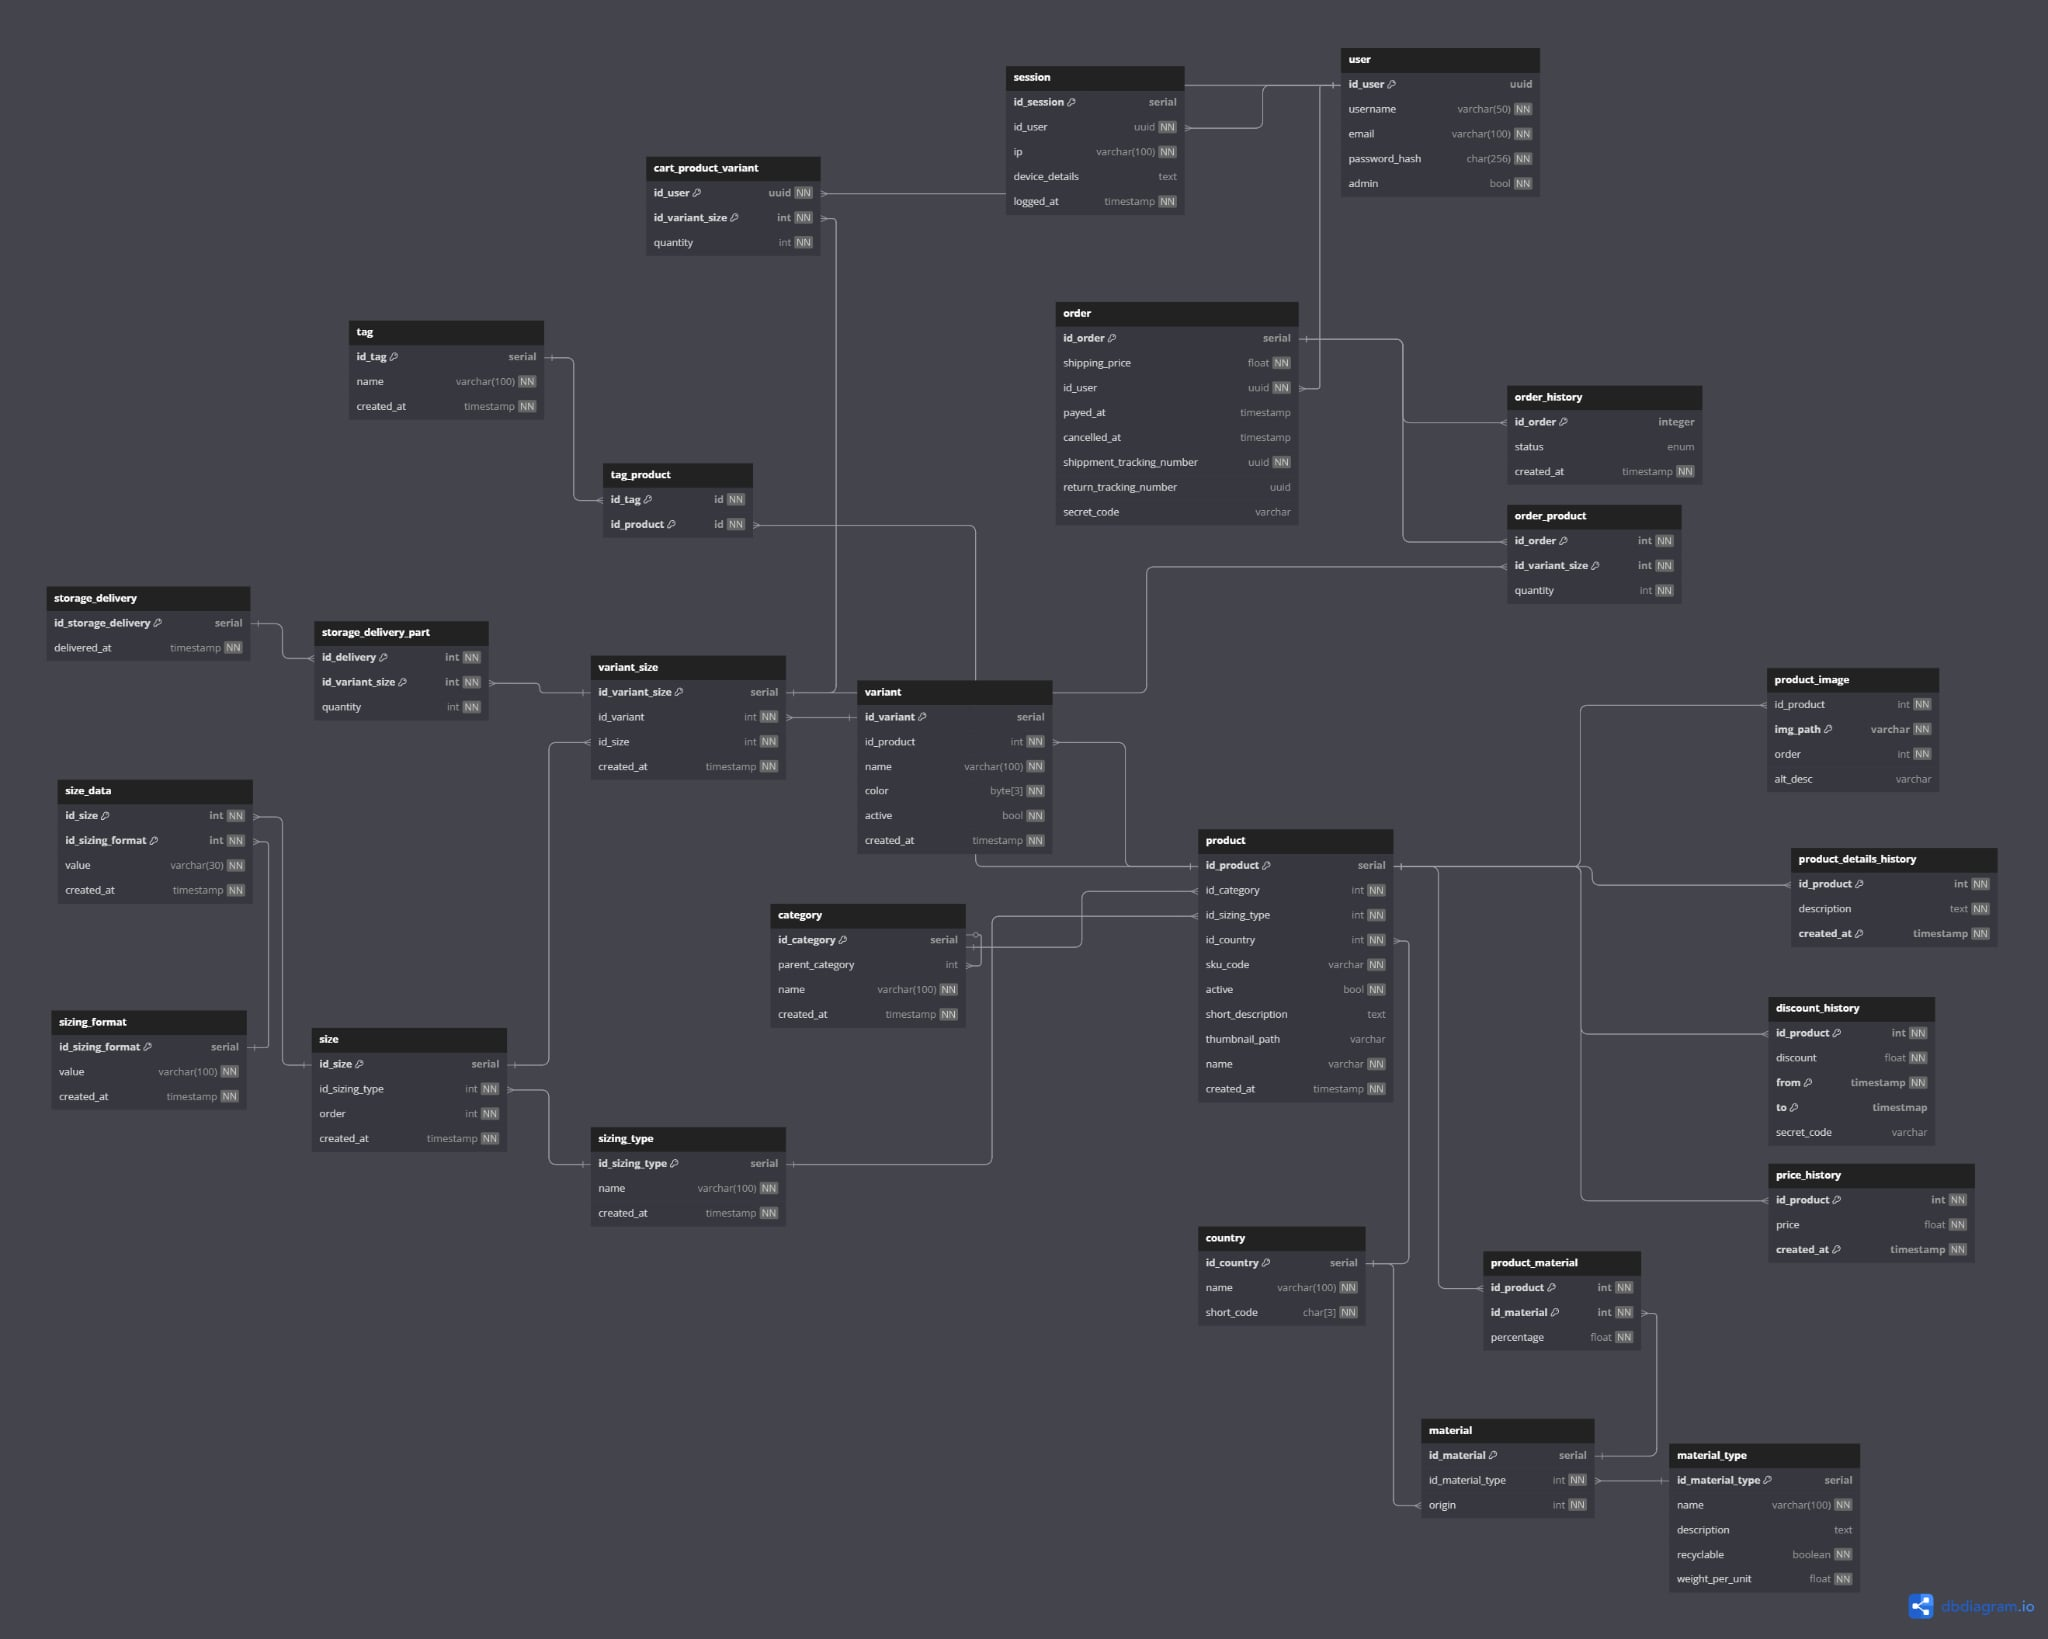
\includegraphics[width=1.0\textwidth]{diagram.jpeg}
    \caption{Diagram bazy danych.}
    \label{fig:database_diagram}
\end{figure}

\section*{Uruchomienie aplikacji}

Aplikacja może być uruchomiona lokalnie przy użyciu Docker Compose:

\begin{enumerate}
    \item Rozpakuj archiwum z kodem źródłowym.
    \item Zainstaluj Docker i Docker Compose.
    \item Przejdź do katalogu projektu.
    \item Uruchom aplikację: \texttt{docker compose up -d --build}
    \item Dostęp do aplikacji: \texttt{http://localhost:8080}
\end{enumerate}

\subsection*{Przykładowe konta użytkowników}

System zawiera wstępnie utworzone konta testowe:

\subsubsection*{Konta zwykłych użytkowników}
\textbf{Email}: 
\begin{itemize}
    \item johnsmith@example.com
    \item janedoe@example.com  
    \item emilyc@example.com
    \item aliceh@example.com
\end{itemize}
\textbf{Hasło}: 12345678

\subsubsection*{Konto administratora}
\textbf{Email}: alexbrown@example.com \\
\textbf{Hasło}: 12345678

\section*{Struktura bazy danych}

Baza danych zawiera ponad 20 tabel zorganizowanych w logiczne grupy:

\subsection*{Użytkownicy i sesje}
\begin{itemize}
    \item \texttt{user} - dane użytkowników z hashowaniem haseł SHA-256
    \item \texttt{session} - sesje użytkowników z informacjami o urządzeniu i IP
\end{itemize}

\subsection*{Produkty i kategorie}
\begin{itemize}
    \item \texttt{product} - podstawowe informacje o produktach z kodem SKU
    \item \texttt{category} - hierarchiczna struktura kategorii (self-referential)
    \item \texttt{variant} - warianty produktów z kolorami (RGB w formacie BYTEA)
    \item \texttt{product\_details\_history} - historia opisów produktów w Markdown
    \item \texttt{price\_history} - historia cen produktów
    \item \texttt{product\_image} - galerie zdjęć produktów
\end{itemize}

\subsection*{System rozmiarów}
\begin{itemize}
    \item \texttt{sizing\_type} - typy rozmiarów (t-shirty, spodnie, buty, itp.)
    \item \texttt{sizing\_format} - formaty reprezentacji (US, EU, UK, International)
    \item \texttt{size} - konkretne rozmiary z kolejnością wyświetlania
    \item \texttt{size\_data} - różne reprezentacje tego samego rozmiaru
    \item \texttt{variant\_size} - dostępne rozmiary dla każdego wariantu
\end{itemize}

\subsection*{Materiały i pochodzenie}
\begin{itemize}
    \item \texttt{material\_type} - typy materiałów z właściwościami (recyklowalność, gęstość)
    \item \texttt{material} - konkretne materiały z krajem pochodzenia
    \item \texttt{product\_material} - skład materiałowy produktów (suma musi być 100\%)
    \item \texttt{country} - kraje z kodami ISO
\end{itemize}

\subsection*{Magazyn i dostawy}
\begin{itemize}
    \item \texttt{storage\_delivery} - dostawy do magazynu
    \item \texttt{storage\_delivery\_part} - szczegóły dostaw dla każdego wariantu
    \item \texttt{storage\_quantity} - aktualne stany magazynowe
\end{itemize}

\subsection*{Zamówienia}
\begin{itemize}
    \item \texttt{order} - główne dane zamówienia z numerami śledzenia
    \item \texttt{order\_history} - historia statusów zamówień (ENUM)
    \item \texttt{order\_product} - produkty w zamówieniach
\end{itemize}

\subsection*{Koszyk i zniżki}
\begin{itemize}
    \item \texttt{cart\_product\_variant} - koszyki użytkowników
    \item \texttt{discount\_history} - historia zniżek z kodami promocyjnymi
    \item \texttt{tag} i \texttt{tag\_product} - system tagowania produktów
\end{itemize}

\section*{Funkcjonalności bazy danych}

\subsection*{Wyzwalacze}
\begin{itemize}
    \item \textbf{Sprawdzanie składu materiałowego} - suma procentów materiałów musi wynosić dokładnie 100\%
    \item \textbf{Spójność typów rozmiarów} - rozmiary dodawane do wariantów muszą być zgodne z typem produktu
\end{itemize}

\subsection*{Funkcje}
\begin{itemize}
    \item \texttt{get\_product\_regular\_price()} - aktualna cena regularna
    \item \texttt{get\_product\_discounted\_price()} - cena z zastosowanymi zniżkami
    \item \texttt{get\_product\_discount\_info()} - informacje o aktywnych zniżkach
    \item \texttt{get\_min\_price\_30\_days()} - najniższa cena z ostatnich 30 dni
    \item \texttt{check\_cart\_availability()} - sprawdzanie dostępności koszyka
    \item \texttt{purchase\_cart()} - atomowe przetwarzanie zakupu
    \item \texttt{calculate\_order\_price\_at\_timestamp()} - kalkulacja cen zamówień historycznych
\end{itemize}

\subsection*{Widoki i reguły}
\begin{itemize}
    \item \texttt{product\_details\_view} - aktualny opis produktu z automatycznym dodawaniem do historii
    \item \texttt{product\_price\_view} - aktualna cena produktu z automatycznym dodawaniem do historii
    \item \texttt{order\_status\_view} - aktualny status zamówienia z automatycznym dodawaniem do historii
\end{itemize}

\subsection*{Indeksy}
Zaimplementowano kompleksowy system indeksów:
\begin{itemize}
    \item \textbf{Wyszukiwanie pełnotekstowe} - GIN na opisach produktów
    \item \textbf{Indeksy częściowe} - tylko dla aktywnych produktów i wariantów
    \item \textbf{Indeksy złożone} - dla popularnych wzorców zapytań
    \item \textbf{Indeksy na klucze obce} - optymalizacja złączeń
\end{itemize}

\section*{System zniżek}

Zaawansowany system rabatów obsługuje:
\begin{itemize}
    \item \textbf{Zniżki ogólne} - bez kodu promocyjnego
    \item \textbf{Zniżki z kodem} - wymagające podania kodu
    \item \textbf{Składanie zniżek} - automatyczne sumowanie rabatów (max 100\%)
    \item \textbf{Zakresy czasowe} - z datami początku i końca
    \item \textbf{Zniżki permanentne} - bez daty końca
\end{itemize}

\section*{Logika aplikacji}

\subsection*{Założenia aplikacji}

Aplikacja została zaprojektowana z uwzględnieniem następujących założeń biznesowych i technicznych:

\subsubsection*{Założenia biznesowe}
\begin{itemize}
    \item \textbf{Darmowa dostawa} - wszystkie zamówienia mają bezpłatną dostawę (shipping\_price = 0)
    \item \textbf{Symulowane płatności} - system płatności zawsze akceptuje transakcje (środowisko demonstracyjne)
    \item \textbf{Niezmienność historyczna} - większość danych po zapisie nie jest modyfikowana, lecz archiwizowana
    \item \textbf{Składanie zniżek} - rabaty mogą się sumować do maksymalnie 100\%
    \item \textbf{Materiały muszą sumować się do 100\%} - skład każdego produktu musi być kompletnie określony
    \item \textbf{Spójność rozmiarów} - warianty produktów mogą mieć tylko rozmiary zgodne z typem produktu
\end{itemize}

\subsubsection*{Założenia techniczne}
\begin{itemize}
    \item \textbf{UUID dla użytkowników} - przygotowanie na przyszłą dystrybucję systemu
    \item \textbf{SERIAL dla pozostałych} - optymalizacja wydajności dla często używanych kluczy
    \item \textbf{Asynchroniczne operacje} - FastAPI z asyncpg dla wysokiej wydajności
    \item \textbf{Hashowanie SHA-256} - bezpieczne przechowywanie haseł
    \item \textbf{Kolory w formacie BYTEA} - efektywne przechowywanie RGB (3 bajty)
    \item \textbf{Parametryzowane zapytania} - ochrona przed SQL injection
\end{itemize}

\section*{Rozwiązane problemy projektowe}

Podczas implementacji udało się rozwiązać kilka kluczowych problemów związanych z projektowaniem sklepu internetowego:

\subsection*{Problemy biznesowe}

\subsubsection*{Złożony system rozmiarów}
\textbf{Problem}: Różne kategorie produktów wymagają różnych systemów rozmiarów (t-shirty: XS-XL, buty: US/EU/UK, dzieci: wiek).

\textbf{Rozwiązanie}: Hierarchiczny system rozmiarów z tabelami:
\begin{itemize}
    \item \texttt{sizing\_type} - typ rozmiaru dla kategorii produktów
    \item \texttt{sizing\_format} - format reprezentacji (US, EU, UK, International)
    \item \texttt{size\_data} - różne reprezentacje tego samego rozmiaru
    \item Wyzwalacz sprawdzający zgodność rozmiarów z typem produktu
\end{itemize}

\subsubsection*{Historyczne kalkulacje cen i zniżek}
\textbf{Problem}: Konieczność zachowania historycznych cen zamówień i możliwość składania różnych typów rabatów.

\textbf{Rozwiązanie}:
\begin{itemize}
    \item Funkcja \texttt{calculate\_order\_price\_at\_timestamp()} - dokładne odtworzenie cen historycznych
    \item System składania zniżek z ograniczeniem do 100\%
    \item Obsługa zniżek ogólnych i z kodami promocyjnymi
    \item Historia wszystkich zmian cen i rabatów
\end{itemize}

\subsubsection*{Kontrola spójności składu materiałowego}
\textbf{Problem}: Zapewnienie, że skład materiałowy każdego produktu sumuje się dokładnie do 100\%.

\textbf{Rozwiązanie}: Wyzwalacz \texttt{trg\_product\_material\_check\_sum()} z mechanizmem DEFERRED CONSTRAINT, pozwalającym na atomowe operacje na składzie materiałowym.

\subsection*{Problemy techniczne}

\subsubsection*{Wydajność zapytań}
\textbf{Problem}: Złożone zapytania łączące wiele tabel mogą być wolne przy dużej ilości danych.

\textbf{Rozwiązanie}:
\begin{itemize}
    \item Strategiczne indeksy częściowe (tylko dla aktywnych produktów)
    \item Indeksy złożone dla popularnych wzorców zapytań
    \item Indeksy GIN dla wyszukiwania pełnotekstowego
    \item Funkcje PL/pgSQL dla skomplikowanych obliczeń
\end{itemize}

\subsubsection*{Atomowość zakupów}
\textbf{Problem}: Zapewnienie, że zakup koszyka jest operacją atomową z kontrolą dostępności.

\textbf{Rozwiązanie}: Funkcja \texttt{purchase\_cart()} z:
\begin{itemize}
    \item Blokowaniem zasobów (FOR UPDATE)
    \item Sprawdzaniem dostępności przed zakupem
    \item Transakcyjnym przenoszeniem danych z koszyka do zamówienia
    \item Automatycznym rollback przy błędach
\end{itemize}

\subsubsection*{Skalowalność systemu sesji}
\textbf{Problem}: Efektywne zarządzanie sesjami użytkowników bez nadmiernego obciążenia bazy.

\textbf{Rozwiązanie}:
\begin{itemize}
    \item Pool połączeń asyncpg (2-10 połączeń)
    \item Asynchroniczne operacje I/O
    \item Minimalizacja czasu blokowania transakcji
    \item Przygotowanie na rozproszone UUID dla użytkowników
\end{itemize}

\subsection*{Niezmienność danych}
Większość danych jest niezmienna po wstawieniu - zamiast modyfikacji tworzona jest historia:
\begin{itemize}
    \item Opisy produktów (\texttt{product\_details\_history})
    \item Ceny produktów (\texttt{price\_history}) 
    \item Statusy zamówień (\texttt{order\_history})
    \item Zniżki (\texttt{discount\_history})
\end{itemize}

\subsection*{System płatności}
\begin{itemize}
    \item Symulowane płatności - zawsze akceptowane
    \item Darmowa dostawa dla wszystkich zamówień
    \item Atomowe przetwarzanie zakupów z kontrolą dostępności
\end{itemize}

\subsection*{Zarządzanie stanem}
\begin{itemize}
    \item Produkty i warianty mogą być oznaczone jako nieaktywne (\texttt{active = false})
    \item Zachowanie historii dla nieaktywnych elementów
    \item Kontrola dostępności na poziomie wariant-rozmiar
\end{itemize}

\section*{Architektura aplikacji}

\subsection*{Backend (FastAPI)}
\begin{itemize}
    \item \textbf{Wzorzec Repository} - abstrakcja dostępu do bazy danych
    \item \textbf{Modele Pydantic} - walidacja i serializacja danych
    \item \textbf{Routery} - obsługa endpointów HTTP i szablonów
    \item \textbf{Middleware CORS} - obsługa zapytań cross-origin
\end{itemize}

\subsection*{Frontend}
\begin{itemize}
    \item \textbf{Szablony Jinja2} - renderowanie HTML
    \item \textbf{Bootstrap 5} - responsywny design
    \item \textbf{JavaScript} - interaktywne elementy (preview zniżek, filtry)
\end{itemize}

\subsection*{Bezpieczeństwo}
\begin{itemize}
    \item Hashowanie haseł SHA-256
    \item Sesje z informacjami o urządzeniu
    \item Rozróżnienie użytkowników zwykłych i administratorów
    \item Parametryzowane zapytania SQL (ochrona przed SQL injection)
\end{itemize}

\section*{Funkcjonalności systemu}

\subsection*{Panel użytkownika}
\begin{itemize}
    \item Rejestracja i logowanie z walidacją
    \item Przeglądanie produktów z filtrami (kategorie, tagi, rozmiary)
    \item Koszyk z kontrolą dostępności
    \item Historia zamówień z kalkulacją rabatów
    \item Możliwość dokonania zwrotu produktów
\end{itemize}

\subsection*{Panel administratora}
\begin{itemize}
    \item Tworzenie nowych produktów z materiałami i tagami
    \item Modyfikacja produktów (opisy, ceny, warianty)
    \item Zarządzanie zniżkami z podglądem produktów
    \item Zarządzanie zamówieniami i statusami
    \item Dodawanie dostaw do magazynu
\end{itemize}

\section*{Dane testowe}

System zawiera bogaty zestaw danych testowych:
\begin{itemize}
    \item 25 produktów w różnych kategoriach
    \item Ponad 60 wariantów kolorystycznych
    \item Kompleksne historie cen i opisów
    \item System zniżek z różnymi rodzajami rabatów
    \item Przykładowe zamówienia i historie statusów
    \item Pełne dane magazynowe
\end{itemize}

\section*{Optymalizacja}

\subsection*{Wydajność bazy danych}
\begin{itemize}
    \item Pool połączeń asyncpg (2-10 połączeń)
    \item Strategiczne indeksy dla krytycznych zapytań
    \item Funkcje PL/pgSQL dla skomplikowanych obliczeń
    \item Widoki materiałowe dla często używanych danych
\end{itemize}

\subsection*{Skalowalność}
\begin{itemize}
    \item Asynchroniczne operacje I/O
    \item Efektywne zarządzanie sesjami
    \item Optymalizacja zapytań z indeksami częściowymi
    \item Przygotowanie na rozproszenie (UUID dla użytkowników)
\end{itemize}

\end{document}

